% 5.whitebox.tex — Experiments

\section{Experiments}
\label{sec:experiments}
\setlength{\emergencystretch}{3em}

\subsection{Setup}
\label{sec:exp_setup}

\paragraph{Target models.}
We evaluate five ALLMs spanning diverse audio pipelines:
\textbf{Voxtral-Mini-3B}~\cite{voxtral} (Whisper encoder--linear adapter--3B Mistral decoder);
\textbf{OpenS2S}~\cite{opens2s} (dedicated speech-understanding module producing a fused semantic--paralinguistic tensor for a Qwen-based LLM);
\textbf{MERaLiON-2-3B}~\cite{meralion} (Whisper-style encoder with explicit paralinguistic supervision);
\textbf{SALMONN-7B}~\cite{salmonn} (dual Whisper+BEATs front end, Q-Former fusion, Vicuna-7B backbone);
\textbf{Kimi-Audio-7B}~\cite{kimiaudio} (proprietary non-Whisper audio tokenizer, 7B LLM).
The five models route emotional information through fundamentally different mechanisms---shared encoder pathway, specialized perception module, paralinguistic-supervised decoder, dual-stream fusion, or separate tokenization---providing a strong generality test.

\paragraph{Dataset and evaluation protocol.}
Experiments span four datasets---ESD-EN, ESD-CN~\cite{esd}, IEMOCAP~\cite{iemocap}, and RAVDESS~\cite{ravdess}---with four source emotions (\texttt{angry}, \texttt{neutral}, \texttt{sad}, \texttt{surprise}) each targeted to \texttt{happy}.
Two scales are used: \textit{full-scale} (Voxtral and OpenS2S on large ESD sweeps plus 60-sample IEMOCAP/RAVDESS subsets) and \textit{matched-subset} (all five models on 60~samples/dataset, 240~total, same seed); Table~\ref{tab:main_results} reports full-scale where available, matched-subset otherwise.
Each adversarial audio is tested under three emotion-elicitation prompts; a sample counts as a targeted success only if $\geq$2 of 3 yield the target emotion.
Semantic preservation is measured by cosine similarity of sentence embeddings (threshold $0.8$); for OpenS2S, an LLM judge (DeepSeek V3~\cite{deepseek}) corroborates at $90.60\%$ agreement.
Following AHa-Bench~\cite{aha-bench}, we also report \textit{semantic-acoustic confusion} (H$_{\text{sac}}$)---the rate at which the attack flips emotion while preserving content.

\paragraph{Attack configuration.}
Perturbation budget: $\varepsilon = 0.008$ ($L_\infty$).
The three-phase design (Section~\ref{sec:methodology}) maps to a two-window schedule: Window~A (20~steps, Phases~I--II) emphasizes $\mathcal{L}_{\mathrm{exit}}$ and $\mathcal{L}_{\mathrm{perc}}$; Window~B (40~steps, Phase~III) balances all losses including $\mathcal{L}_{\mathrm{comp}}$.
Convergence: emotion loss $<1.0$; multi-prompt ensemble and EoT augmentation are applied throughout.


%%% ----------------------------------------------------------------
\subsection{Targeted Emotion Flipping}
\label{sec:exp_asr}

\begin{table*}[!t]
\centering
\small
\caption{White-box targeted emotion flipping results across five models and four datasets.
Targeted ASR (\%) is determined by majority vote over three emotion elicitation prompts.
Hallucination metrics follow the AHa-Bench~\cite{aha-bench} framework:
ACC = overall perception accuracy on adversarial audio (emotion probes $+$ semantic probe); $\Delta$ACC = accuracy drop from clean to adversarial; H$_{\text{sem}}$ = semantic hallucination rate; H$_{\text{sac}}$ = semantic-acoustic confusion rate (emotion flipped $\wedge$ semantic preserved).
All values are percentages; top results per column in \textbf{bold}; ``---'' = hallucination evaluation pending.}
\label{tab:main_results}
\setlength{\tabcolsep}{5pt}
\begin{tabular}{l cccc c cccc}
\toprule
 & \multicolumn{5}{c}{\textbf{Targeted ASR (\%) $\uparrow$}} & \multicolumn{4}{c}{\textbf{Adversarial Hallucination (\%)}} \\
\cmidrule(lr){2-6} \cmidrule(lr){7-10}
\textbf{Models} & IEMOCAP & RAVDESS & ESD-EN & ESD-CN & Avg & ACC$\downarrow$ & $\Delta$ACC$\uparrow$ & H$_{\text{sem}}$$\uparrow$ & H$_{\text{sac}}$$\uparrow$ \\
\midrule
Voxtral-Mini-3B & 96.67 & 96.67 & 91.40 & 96.20 & 95.24 & 10.8 & 35.9 & 59.2 & 37.5 \\
OpenS2S         & 91.67 & 93.33 & 94.40 & 77.40 & 89.20 & \textbf{5.5} & \textbf{66.6} & \textbf{78.3} & 19.4 \\
MERaLiON-2-3B   & \textbf{100.00} & \textbf{100.00} & \textbf{100.00} & \textbf{100.00} & \textbf{100.00} & 12.6 & 41.7 & 49.7 & \textbf{50.3} \\
SALMONN-7B      & 90.37 & 86.24 & 92.75 & 81.36 & 87.67 & --- & --- & --- & --- \\
Kimi-Audio-7B   & 93.53 & 94.21 & 91.22 & 85.78 & 91.53 & --- & --- & --- & --- \\
\bottomrule
\end{tabular}
\end{table*}

The left half of Table~\ref{tab:main_results} reports targeted ASR.
Under $L_\infty{=}0.008$---$3.75{\times}$ smaller than the SER baselines of Section~\ref{sec:obs_q3} (none exceeding $10.5\%$ untargeted change)---the 3-prompt majority-vote ASR reaches $95.24\%$ (Voxtral), $89.20\%$ (OpenS2S), $100.00\%$ (MERaLiON), $87.67\%$ (SALMONN), and $91.53\%$ (Kimi-Audio).
A budget inert for traditional SER attacks thus suffices for near-complete targeted emotion control once the attack targets the autoregressive pipeline.

Cross-model variation tracks how each architecture processes emotional cues rather than model size.
Voxtral's diffuse encoder--adapter representations yield easy redirection ($99.90\%$ convergence, mean $5.4$ steps).
OpenS2S's dedicated perception module creates a compact, harder-to-move boundary: only $47.85\%$ converge (mean $39.5$ steps), explaining its lower ASR---especially on ESD-CN ($77.40\%$).
MERaLiON's paralinguistic-supervised decoder concentrates emotion in a locally sharp pathway---$100\%$ convergence with trivial cost.
SALMONN ($87.67\%$) and Kimi-Audio ($91.53\%$) fall between; both show a Mandarin dip (ESD-CN: $81.36\%$, $85.78\%$), consistent with language-dependent prosodic cues being harder to perturb.


\begin{figure}[!t]
\centering
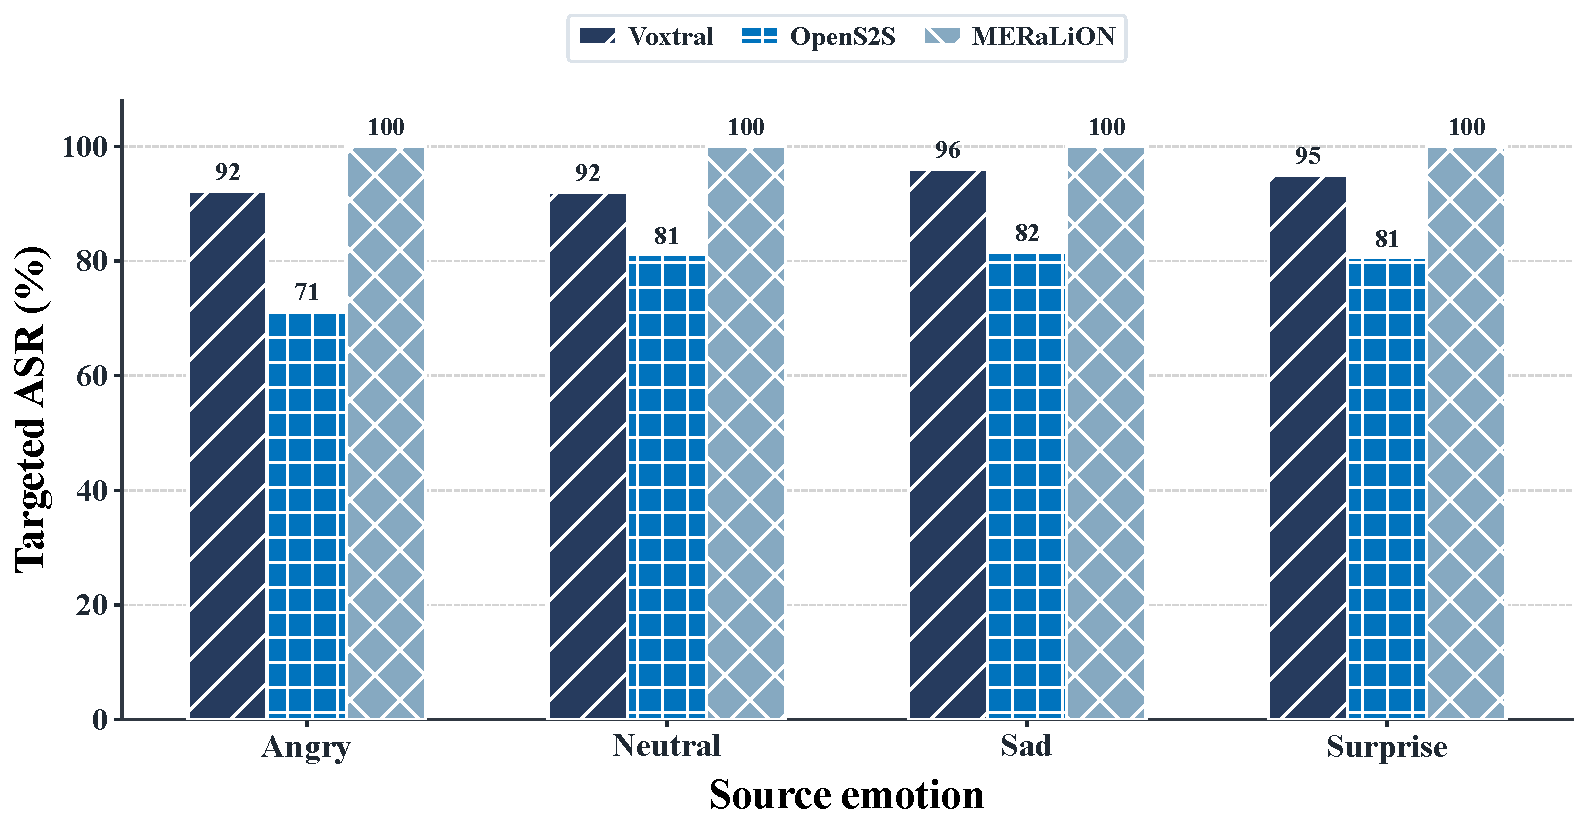
\includegraphics[width=\columnwidth]{figure/fig_exp_per_emotion_asr.pdf}
\caption{Per-emotion targeted ASR (\%, majority vote) on the matched-subset pool.
Source emotion is the ground-truth label of the clean audio, and the attack target is \texttt{happy}.
The complete five-model table is moved to Appendix~Table~\ref{tab:app_per_emotion_asr}.}
\label{fig:exp_per_emotion_asr}
\end{figure}

\paragraph{Per-emotion analysis.}
Figure~\ref{fig:exp_per_emotion_asr} visualizes ASR by source emotion on the matched subset.
Voxtral shows a tight range ($92$--$96\%$); OpenS2S exhibits wider spread with \texttt{angry} hardest ($71.21\%$) and \texttt{sad}/\texttt{neutral} exceeding $81\%$---consistent with the competition-field analysis of Section~\ref{sec:clean-emotion-observation}, where \texttt{angry} acts as a dominant competitor resisting displacement while \texttt{sad} provides clearer gradient handles.
MERaLiON flips every sample regardless of source emotion, pointing to a decision boundary that is locally sharp but globally fragile along the \texttt{happy} direction.


%%% ----------------------------------------------------------------
\subsection{Cross-Model Transferability}
\label{sec:exp_transfer}

A more deployment-relevant question is whether adversarial waveforms crafted against one model retain targeted effect on a \emph{different} model.
For each source--target pair $(S,T)$, 240~adversarial waveforms (60/dataset) from the white-box attack on~$S$ are fed to~$T$'s 3-prompt majority-vote classifier; diagonal cells reproduce white-box ASR.
SALMONN and Kimi-Audio report outgoing transfer only; incoming evaluations are pending.

\begin{table*}[!t]
\centering
\small
\caption{Cross-model transferability of white-box adversarial audio (targeted ASR, \%, majority vote).
Rows = source (attacker); columns = target (evaluator).
Diagonal cells (shaded, italics) = white-box upper bound.
``Avg.\ transfer'' and ``Avg.\ as target'' average the available off-diagonal cells per row/column.
\textbf{Bold} in each column = highest off-diagonal ASR (strongest attacker for that target); in Avg.\ transfer = highest row; in Avg.\ as target = lowest column (most resistant).
``---'' = not yet evaluated.}
\label{tab:cross_model_transfer}
\setlength{\tabcolsep}{6pt}
\begin{tabular}{l ccccc c}
\toprule
 & \multicolumn{5}{c}{\textbf{Target model (evaluator) $\rightarrow$}} & \\
\cmidrule(lr){2-6}
\textbf{Source model (attacker) $\downarrow$}
 & Voxtral & OpenS2S & MERaLiON & SALMONN & Kimi-Audio & \textbf{Avg.\ transfer} \\
\midrule
Voxtral-Mini-3B  & \cellcolor{gray!15}\textit{95.24} & 34.17 & \textbf{29.58} & --- & --- & 31.88 \\
OpenS2S          & 35.42 & \cellcolor{gray!15}\textit{89.20} & 9.58  & --- & --- & 22.50 \\
MERaLiON-2-3B    & 67.79 & 39.25 & \cellcolor{gray!15}\textit{100.00} & --- & --- & \textbf{53.52} \\
SALMONN-7B       & \textbf{75.45} & \textbf{56.89} & 18.45 & \cellcolor{gray!15}\textit{87.67} & --- & 50.26 \\
Kimi-Audio-7B    & 64.37 & 45.77 & 22.75 & --- & \cellcolor{gray!15}\textit{91.53} & 44.30 \\
\midrule
\textbf{Avg.\ as target} & 60.76 & 44.02 & \textbf{20.09} & --- & --- & --- \\
\bottomrule
\end{tabular}
\end{table*}

Three patterns emerge from Table~\ref{tab:cross_model_transfer}.

\textit{(1) Paralinguistic supervision produces strong surrogates but robust targets.}
MERaLiON's incoming column averages only $20.09\%$---less than half of Voxtral's $60.76\%$---making it the hardest to fool via surrogates.
On the outgoing side, paralinguistic-trained models dominate: MERaLiON ($53.52\%$) and SALMONN ($50.26\%$) versus Voxtral ($31.88\%$) and OpenS2S ($22.50\%$).
Gradients from paralinguistic-supervised boundaries carry stronger emotional signals legible to other models, while their narrow vulnerability cones resist incoming transfer.

\textit{(2) Encoder family governs transfer magnitude.}
The top cell is SALMONN\,$\rightarrow$\penalty0\,Voxtral ($75.45\%$); both share Whisper-family front ends.
Crossing encoder families incurs a consistent penalty: MERaLiON\,$\rightarrow$\penalty0\,OpenS2S drops to $39.25\%$ and OpenS2S\,$\rightarrow$\penalty0\,MERaLiON collapses to $9.58\%$---the lowest non-trivial cell, cautioning against Qwen2-Audio-style surrogates for Whisper-family targets.

\textit{(3) Practical surrogate selection.}
The matrix suggests: \emph{match the target's audio front end and prefer a paralinguistic-supervised source}.
SALMONN is a natural candidate for Whisper-derived targets, though this awaits confirmation from pending incoming evaluations.


%%% ----------------------------------------------------------------
\subsection{Adversarial Hallucination Analysis}
\label{sec:exp_quality}

The right panel of Table~\ref{tab:main_results} adopts the AHa-Bench~\cite{aha-bench} hallucination taxonomy, reporting four metrics for the three models with completed evaluation.

ACC collapses to $5.5$--$12.6\%$ across all three models.
The accuracy drop $\Delta$ACC isolates the causal hallucination load: OpenS2S suffers the steepest drop ($66.6\%$), nearly doubling Voxtral's ($35.9\%$); MERaLiON's moderate $41.7\%$ despite $100\%$ emotion flip reflects an already-imperfect clean baseline.
H$_{\text{sem}}$ correlates with optimization dynamics: OpenS2S's slow convergence ($\sim$40 steps) drifts perturbations into content-bearing dimensions ($78.3\%$), while MERaLiON's near-instant convergence limits collateral damage ($49.7\%$).

The most operationally relevant metric is H$_{\text{sac}}$---emotion flip with semantic preservation.
MERaLiON leads ($50.3\%$), Voxtral follows ($37.5\%$), OpenS2S achieves only $19.4\%$ due to heavy semantic damage.
H$_{\text{sem}}$ and H$_{\text{sac}}$ are inversely correlated: defending against semantic hallucination alone does not reduce---and may worsen---the risk of stealthy emotion manipulation.


%%% ---------------------------------------------------------------

\subsection{Black-box Transferability}
\label{sec:exp_blackbox}

In real-world attack scenarios, the target ALLMs usually remain inaccessible to the attacker.
To demonstrate the effectiveness of the proposed emotion attack under such settings, we construct adversarial audio on open-source surrogate ALLMs and evaluate its transferability on closed-source commercial audio-language systems.
This setting is substantially more challenging than white-box evaluation because the target architectures, parameters, system prompts, and mitigation strategies are all unknown to the attacker.
Commercial providers may additionally deploy input filtering or multimodal safeguards, which further raises the bar for successful transfer.

\subsubsection{Attacking Commercial Base Models}

\paragraph{Experimental setup.}
We currently report four completed transferred attack pools obtained from the white-box stage: Voxtral EN ($n=914$), Voxtral CN ($n=962$), OpenS2S EN ($n=944$), and OpenS2S CN ($n=774$).
To support the next round of black-box expansion, we also reserve additional surrogate entries for SALMONN and Kimi-Audio, which can be filled once their corresponding offline attack pools are ready.
The black-box targets currently include four completed commercial base-model APIs---Gemini~2.5~Flash, Gemini~2.5~Pro, Qwen3-Omni-Flash, and Qwen-Omni-Turbo---and one reserved external interface target, Grok Voice Agent API, which will be filled once the corresponding evaluation run is completed.
For each adversarial audio, we query the target model through its external interface, normalize the returned emotion prediction into the four-way label space $\{\texttt{angry}, \texttt{sad}, \texttt{neutral}, \texttt{surprise}\}$, and count a transfer success when the predicted label matches the attacker-specified target emotion.
We also evaluate the paired clean audio on the same interface, which allows us to separate transfer success from target-side prior bias.
OpenAI \texttt{gpt-audio} is excluded from the final table because the corresponding API key was unavailable during the large-scale run.

\begin{figure*}[!t]
\centering
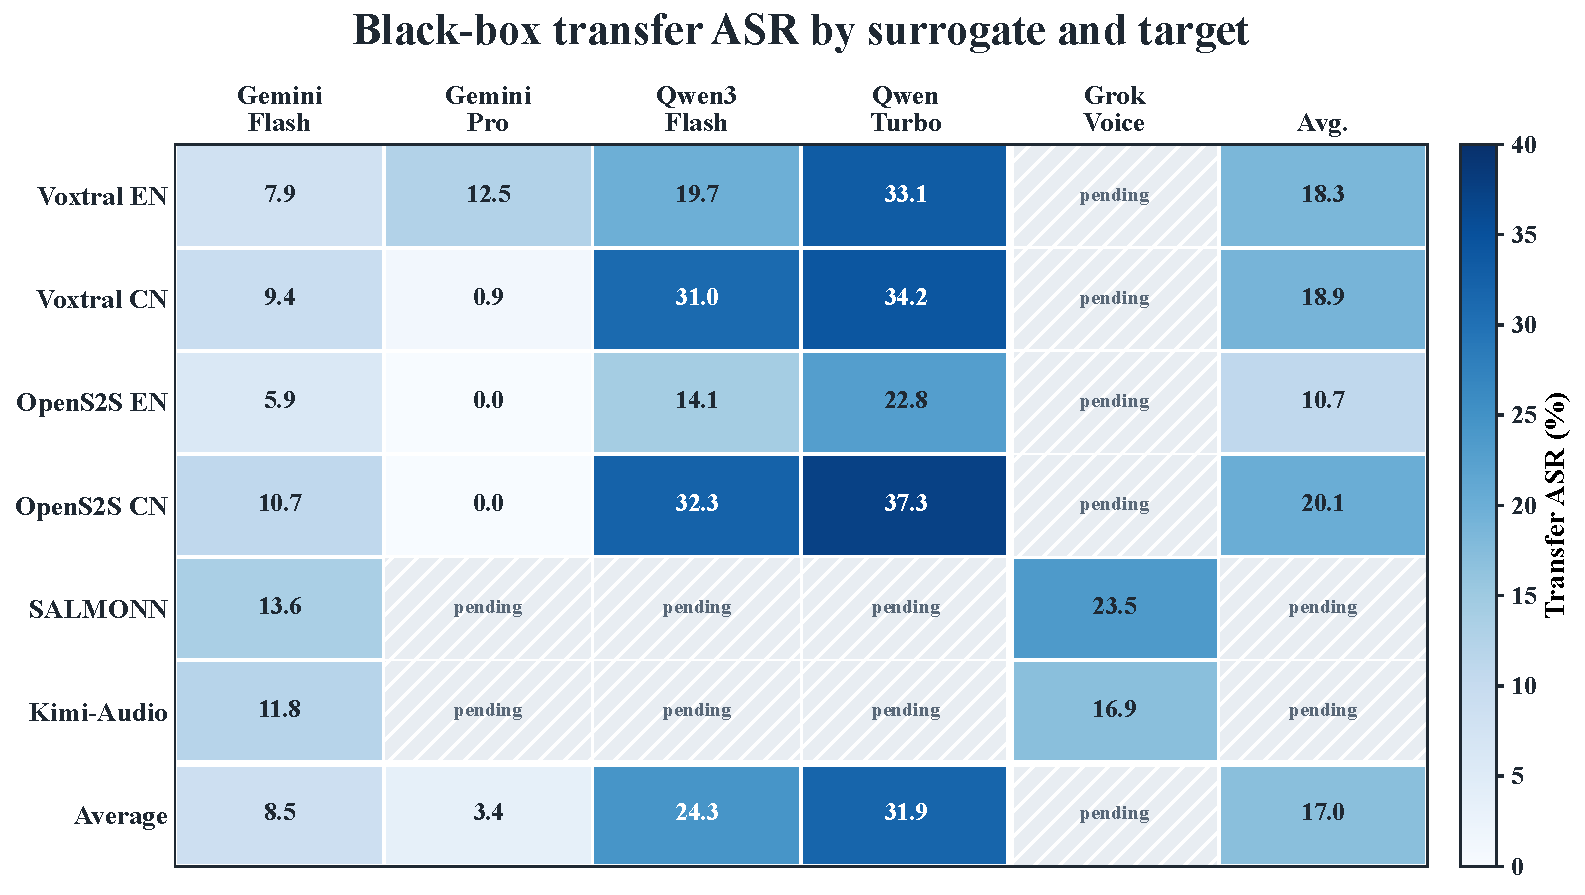
\includegraphics[width=0.82\textwidth]{figure/fig_exp_blackbox_heatmap.pdf}
\caption{Transfer-based black-box targeted ASR (\%) on commercial audio-language targets.
Rows denote the surrogate pool used to generate adversarial audio offline; columns denote the external black-box target.
The average row and column aggregate completed surrogate pools and completed target columns only; hatched cells denote pending evaluations.}
\label{fig:exp_blackbox_heatmap}
\end{figure*}

 \paragraph{Emotion classification task.}
In our experimental setup, we take the adversarial audio generated on the four surrogate pools and evaluate its transferability on the completed commercial base models above, while reserving the Grok Voice Agent API column for the next evaluation round.
The results are visualized in Figure~\ref{fig:exp_blackbox_heatmap}.
The attack demonstrates clear transferability across target families: even without access to the victim's internals, transferred adversarial audio still achieves nontrivial targeted success on all completed black-box targets.
The most vulnerable target is Qwen-Omni-Turbo, which reaches an average transfer ASR of $\mathbf{31.87\%}$ across surrogate pools, while the most robust target is Gemini~2.5~Pro at only $\mathbf{3.35\%}$.
The strongest individual transfer path is OpenS2S CN $\rightarrow$ Qwen-Omni-Turbo at $\mathbf{37.34\%}$.
Although these numbers are lower than the corresponding white-box ASRs in Table~\ref{tab:main_results}, they remain substantial given that the attacker performs no target-specific adaptation and interacts only through the public inference interface.

\paragraph{Target-family dependence.}
The most striking pattern in Figure~\ref{fig:exp_blackbox_heatmap} is that transfer success depends far more on the black-box target family than on the particular surrogate.
Both Qwen targets are consistently more vulnerable than both Gemini targets, regardless of whether the transferred samples originate from Voxtral or OpenS2S, and regardless of language.
This suggests that the transfer phenomenon is not merely due to surrogate overfitting; rather, different commercial model families appear to induce different external emotion decision geometries, some of which are substantially easier to perturb than others.
In particular, the transferability is stronger within the Qwen family, possibly because the external decision behavior of the target model remains better aligned with the surrogate-side emotion boundary.

\paragraph{Clean-to-adversarial gap.}
The black-box transfer effect cannot be explained away by a high clean target prior.
For example, OpenS2S CN $\rightarrow$ Qwen-Omni-Turbo achieves $37.34\%$ ASR even though the paired clean target rate is only $7.62\%$; similarly, Voxtral EN $\rightarrow$ Gemini~2.5~Pro reaches $12.47\%$ ASR from a $0.00\%$ clean target rate.
Across the completed target models, adversarial audio therefore changes the emotion decision far more often than would be expected from the target system's clean-side confusion alone.
This gap is important because it shows that transfer is not just exploiting pre-existing black-box ambiguity; it is actively steering the target model toward the attacker-specified emotion.

\paragraph{Per-emotion transfer patterns.}
Transfer is also strongly emotion-dependent.
Across multiple surrogate--target combinations, \texttt{surprise} is the easiest target to transfer, whereas \texttt{neutral} is typically the hardest.
For instance, OpenS2S CN $\rightarrow$ Qwen-Omni-Turbo reaches $58.13\%$ on \texttt{surprise} but only $28.43\%$ on \texttt{neutral}; Voxtral CN $\rightarrow$ Qwen-Omni-Turbo shows a similar pattern with $54.92\%$ versus $25.94\%$.
This asymmetry mirrors the white-box observation that emotion classes occupy unequal and nonuniform regions in the model's internal competition field.
The fact that the same high-level ordering reappears under black-box transfer suggests that these emotion-specific vulnerabilities are not tied to a single architecture, but reflect a broader property of audio-language emotion processing.

\paragraph{Language effect.}
Cross-lingual conditions also matter, although less strongly than target-family dependence.
On both Qwen targets, Chinese surrogate pools are consistently more transferable than English pools: for example, Voxtral CN exceeds Voxtral EN by $11.29$ points on Qwen3-Omni-Flash, while OpenS2S CN exceeds OpenS2S EN by $18.21$ points on the same target and by $14.56$ points on Qwen-Omni-Turbo.
On Gemini, however, the language effect is weaker and less stable, and in one Voxtral-based setting it even reverses.
This discrepancy suggests that language is not a universal multiplier of transferability; rather, it interacts with the target family and with the surrogate-side acoustic regularities.
In practical terms, the result implies that a black-box attacker may be able to increase transfer yield not only by changing the surrogate architecture, but also by choosing a surrogate language regime that better matches the victim's external emotion interface.

\paragraph{Toward pure black-box optimization.}
The results above focus on zero-shot transfer, where adversarial audio is generated fully offline on open-source surrogates and then directly replayed on the victim target.
For previously unseen black-box models such as new ChatGPT- or Gemini-style audio interfaces, the same framework can be extended to a stronger \emph{pure black-box} setting with limited target queries.
In practice, the attacker would first use a small clean probe set to profile the target's coarse emotion interface---for example, its dominant bias direction, language sensitivity, and the source--target pairs that are easiest to flip---then select or reweight the most compatible surrogate pools accordingly.
After this target profiling stage, one can further refine the transferred waveform with query-efficient score-based search in a low-dimensional perturbation subspace derived from successful white-box attacks, without requiring gradients or target-side internals.
We leave the full empirical evaluation of this pure black-box extension to future work, but include it here to clarify how the current transfer-based setting can naturally scale toward target-aware black-box adaptation.

\subsubsection{Toward Platform-hosted Custom Agents}

\begin{figure}[!t]
\centering
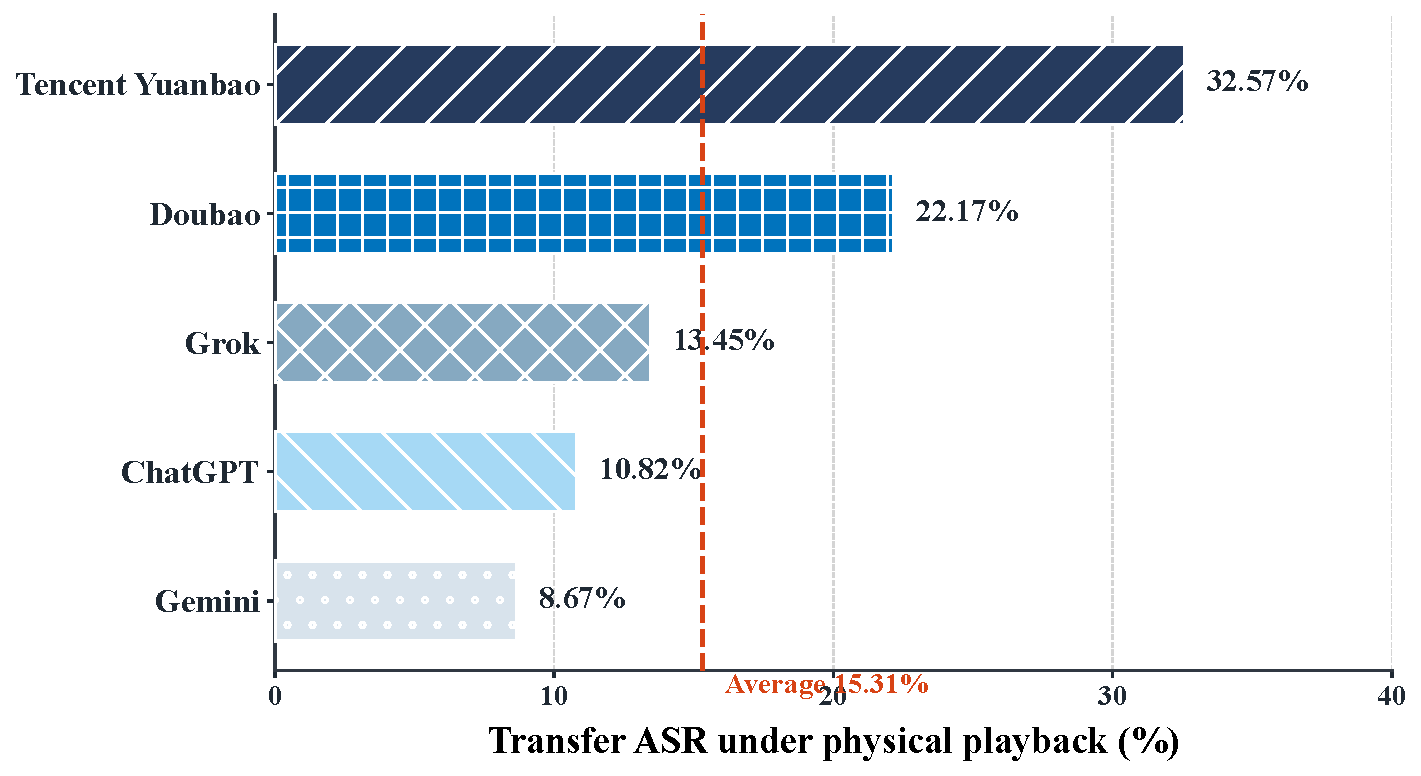
\includegraphics[width=\columnwidth]{figure/fig_exp_platform_agents.pdf}
\caption{Transfer-based ASR (\%) on platform-hosted custom agents under over-the-air physical playback.
Unlike the API-based base-model evaluation above, these targets are tested through real voice-facing product interfaces, so the results include acoustic propagation, replay-record distortion, and platform-specific orchestration effects.}
\label{fig:exp_platform_agents}
\end{figure}

Beyond commercial base models, we further evaluate platform-hosted custom agents, which better reflect what end users actually interact with in real deployment settings.
This setting is intentionally stronger than the API-based black-box evaluation above.
For commercial base models, the adversarial waveform is fed to the target through a direct software interface; by contrast, for platform-hosted agents we evaluate the attack under \emph{physical-layer over-the-air playback}.
That is, the adversarial audio is replayed by a loudspeaker, propagates through air, and is then captured by the target platform's microphone / application frontend before reaching the hosted agent itself.
Compared with base-model APIs, these systems therefore add two additional barriers at once: an acoustic replay channel and an orchestration layer consisting of platform wrappers, hidden role prompts, frontend preprocessing, and agent-specific response policies.

Figure~\ref{fig:exp_platform_agents} shows that the transferred attack remains effective even under this more realistic end-to-end setting.
Among the evaluated platforms, Tencent Yuanbao is the most vulnerable at $\mathbf{32.57\%}$ ASR, followed by Doubao at $\mathbf{22.17\%}$.
By contrast, ChatGPT ($10.82\%$) and Gemini ($8.67\%$) are markedly more robust, while Grok remains moderately vulnerable at $13.45\%$.
The average ASR across the five platform-hosted agents is $15.31\%$, indicating that the vulnerability discovered in white-box speech models is not confined to base commercial models, but can further propagate into realistic hosted-agent ecosystems after passing through physical replay and product-layer mediation.

This result is important because it rules out a simpler interpretation of black-box transfer as a purely interface-level artifact.
If the effect disappeared as soon as the signal left the digital API channel, one could argue that the vulnerability depended on a fragile software path.
Instead, the persistence of nontrivial ASR under over-the-air replay shows that the attack can survive loudspeaker playback, air-channel distortion, device capture, and platform-side preprocessing before the hosted agent makes its final emotion judgment.

\paragraph{Black-box take-away.}
Taken together, these results extend the white-box findings in two ways.
First, they show that emotion-targeted adversarial audio remains effective after deployment, even when the attacker has no access to model internals and performs no target-aware optimization.
Second, they reveal that transfer success is structured rather than random: it depends on target family, emotion direction, and surrogate language.
The black-box evidence therefore supports a stronger claim than white-box feasibility alone: emotion vulnerabilities in ALLMs are not confined to laboratory access assumptions, but can survive not only in realistic API-facing systems, but also in physical over-the-air product interfaces.
